\documentclass[a4paper]{oblivoir}
\usepackage{amsmath,amssymb,kotex,mdframed,tabto,paralist,graphicx}
\usepackage{fapapersize}
\usefapapersize{210mm,297mm,10mm,*,10mm,*}

%%% Counters
\newcounter{num}

%%% Commands
\newcommand\defi[1]
{\bigskip\par\noindent\stepcounter{num} \textbf{정의 \thenum) #1}\par\noindent}
\newcommand\theo[1]
{\bigskip\par\noindent\stepcounter{num} \textbf{정리 \thenum) #1}\par\noindent}
\newcommand\exam[1]
{\bigskip\par\noindent\stepcounter{num} \textbf{예시 \thenum) #1}\par\noindent}
\newcommand\prob[1]
{\bigskip\par\noindent\stepcounter{num} \textbf{문제 \thenum) #1}\par\noindent}

\newcommand\pb[1]{\ensuremath{\fbox{\phantom{#1}}}}

\newcommand\ba{\ensuremath{\:|\:}}

\newcommand\procedure[1]{\begin{mdframed}\vspace{#1\textheight}\end{mdframed}\bigskip}

\newcommand\an[1]{\bigskip\par\noindent\textbf{문제 #1)}\par\noindent}

%%% Meta Commands
\let\oldsection\section
\renewcommand\section{\clearpage\oldsection}

\let\emph\textsf

% 길이 일괄조정
\newlength{\frameheight}
\setlength{\frameheight}{6cm}  % 여기서 높이를 일괄 조절

\newlength{\imagewidth}
\setlength{\imagewidth}{0.38\textwidth}  % 이미지 너비 조절

\begin{document}
\par\bigskip
a. 기울기가 $3$이고 $(2,1)$을 지나는 직선의 방정식을 구하여라.\par
\begin{minipage}{0.45\textwidth}\centering
\par\bigskip\begin{mdframed}[frametitle=중학교 방식의 풀이]
\vspace{\frameheight}
\end{mdframed}
\end{minipage}
\begin{minipage}{0.45\textwidth}\centering
\par\bigskip\begin{mdframed}[frametitle=공식을 사용한 풀이]
\vspace{\frameheight}
\end{mdframed}
\end{minipage}\bigskip\bigskip\par
\par\bigskip
b. 기울기가 $2$이고 $(1,5)$을 지나는 직선의 방정식을 구하여라.\par
\begin{minipage}{0.45\textwidth}\centering
\par\bigskip\begin{mdframed}[frametitle=중학교 방식의 풀이]
\vspace{\frameheight}
\end{mdframed}
\end{minipage}
\begin{minipage}{0.45\textwidth}\centering
\par\bigskip\begin{mdframed}[frametitle=공식을 사용한 풀이]
\vspace{\frameheight}
\end{mdframed}
\end{minipage}\bigskip\bigskip\par
\par\bigskip
c. 기울기가 $-1$이고 $(3,5)$을 지나는 직선의 방정식을 구하여라.\par
\begin{minipage}{0.45\textwidth}\centering
\par\bigskip\begin{mdframed}[frametitle=중학교 방식의 풀이]
\vspace{\frameheight}
\end{mdframed}
\end{minipage}
\begin{minipage}{0.45\textwidth}\centering
\par\bigskip\begin{mdframed}[frametitle=공식을 사용한 풀이]
\vspace{\frameheight}
\end{mdframed}
\end{minipage}\bigskip\bigskip\par

\newpage
\par\bigskip
d. 기울기가 $1$이고 $(-2,3)$을 지나는 직선의 방정식을 구하여라.\par
\begin{minipage}{0.45\textwidth}\centering
\par\bigskip\begin{mdframed}[frametitle=중학교 방식의 풀이]
\vspace{\frameheight}
\end{mdframed}
\end{minipage}
\begin{minipage}{0.45\textwidth}\centering
\par\bigskip\begin{mdframed}[frametitle=공식을 사용한 풀이]
\vspace{\frameheight}
\end{mdframed}
\end{minipage}\bigskip\bigskip\par
\par\bigskip
e. 기울기가 $\frac12$이고 $(4,1)$을 지나는 직선의 방정식을 구하여라.\par
\begin{minipage}{0.45\textwidth}\centering
\par\bigskip\begin{mdframed}[frametitle=중학교 방식의 풀이]
\vspace{\frameheight}
\end{mdframed}
\end{minipage}
\begin{minipage}{0.45\textwidth}\centering
\par\bigskip\begin{mdframed}[frametitle=공식을 사용한 풀이]
\vspace{\frameheight}
\end{mdframed}
\end{minipage}\bigskip\bigskip\par
\par\bigskip
f. 기울기가 $-\frac23$이고 $(-6,0)$을 지나는 직선의 방정식을 구하여라.\par
\begin{minipage}{0.45\textwidth}\centering
\par\bigskip\begin{mdframed}[frametitle=중학교 방식의 풀이]
\vspace{\frameheight}
\end{mdframed}
\end{minipage}
\begin{minipage}{0.45\textwidth}\centering
\par\bigskip\begin{mdframed}[frametitle=공식을 사용한 풀이]
\vspace{\frameheight}
\end{mdframed}
\end{minipage}\bigskip\bigskip\par

\newpage
\par\bigskip
g. 기울기가 $3$이고 $y$절편이 $1$인 직선의 방정식을 구하여라.\par
\begin{minipage}{0.45\textwidth}\centering
\par\bigskip\begin{mdframed}
\vspace{\frameheight}
\end{mdframed}
\end{minipage}
\begin{minipage}{0.45\textwidth}\centering
\par\bigskip\par\bigskip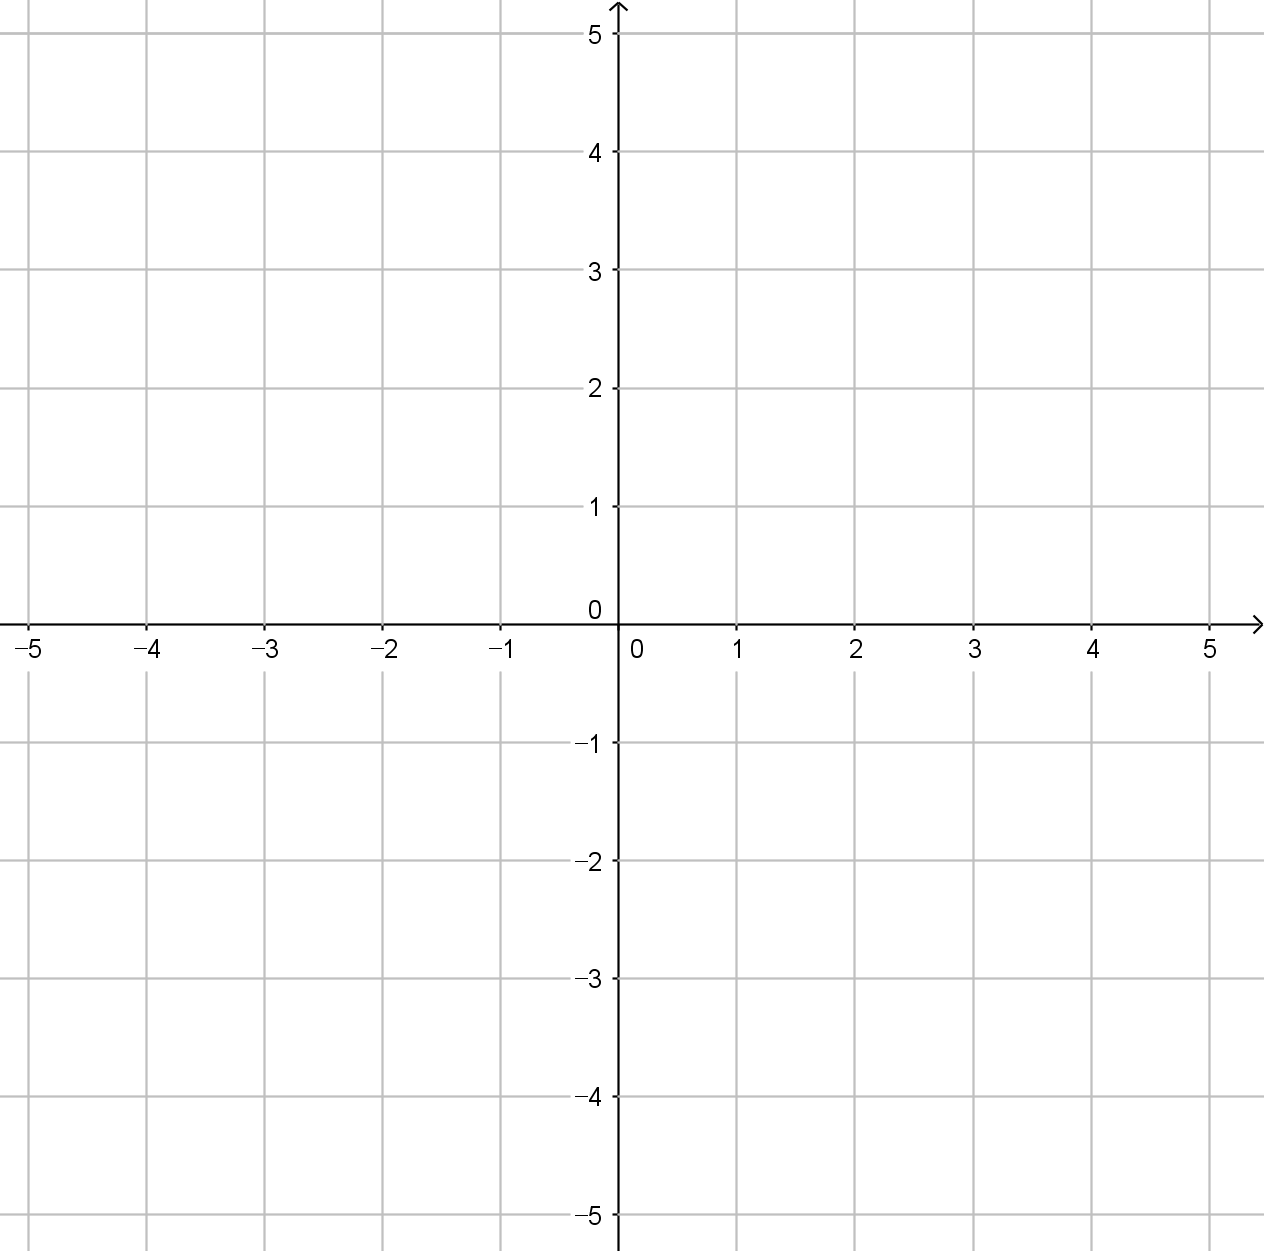
\includegraphics[width=\imagewidth]{55}
\end{minipage}\bigskip\bigskip\par
\par\bigskip
h. 기울기가 $2$이고 $x$절편이 $4$인 직선의 방정식을 구하여라.\par
\begin{minipage}{0.45\textwidth}\centering
\par\bigskip\begin{mdframed}
\vspace{\frameheight}
\end{mdframed}
\end{minipage}
\begin{minipage}{0.45\textwidth}\centering
\par\bigskip\par\bigskip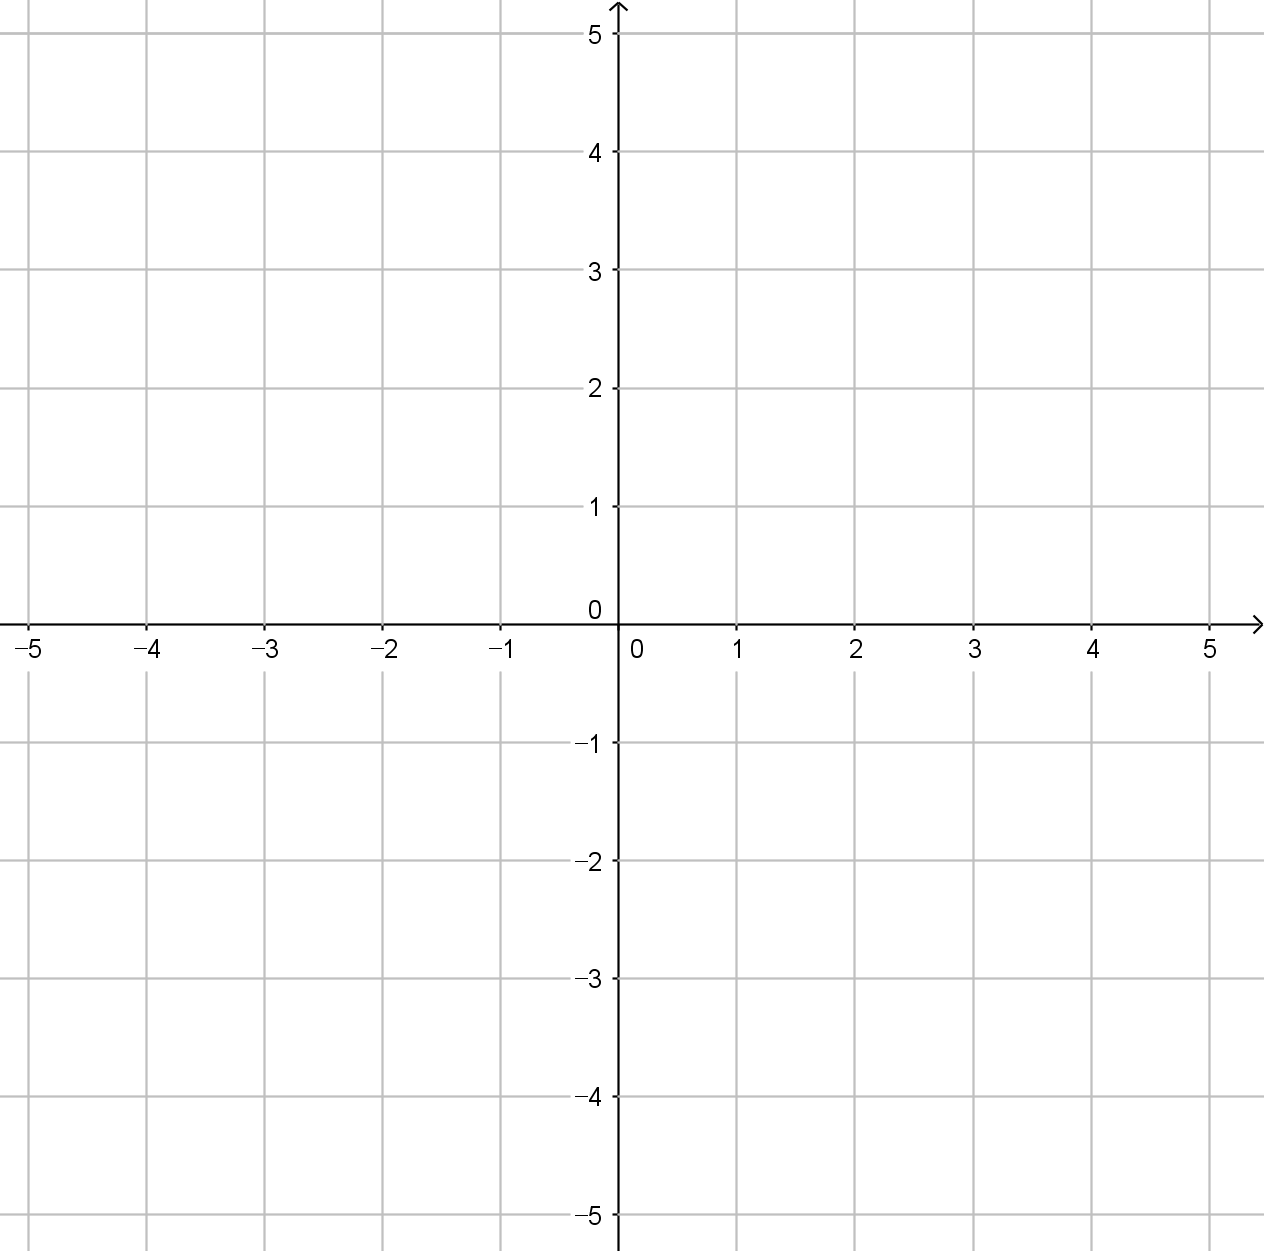
\includegraphics[width=\imagewidth]{55}
\end{minipage}\bigskip\bigskip\par
\par\bigskip
i. $x$절편이 $-2$이고 $y$절편이 4인 직선의 방정식을 구하여라.\par
\begin{minipage}{0.45\textwidth}\centering
\par\bigskip\begin{mdframed}
\vspace{\frameheight}
\end{mdframed}
\end{minipage}
\begin{minipage}{0.45\textwidth}\centering
\par\bigskip\par\bigskip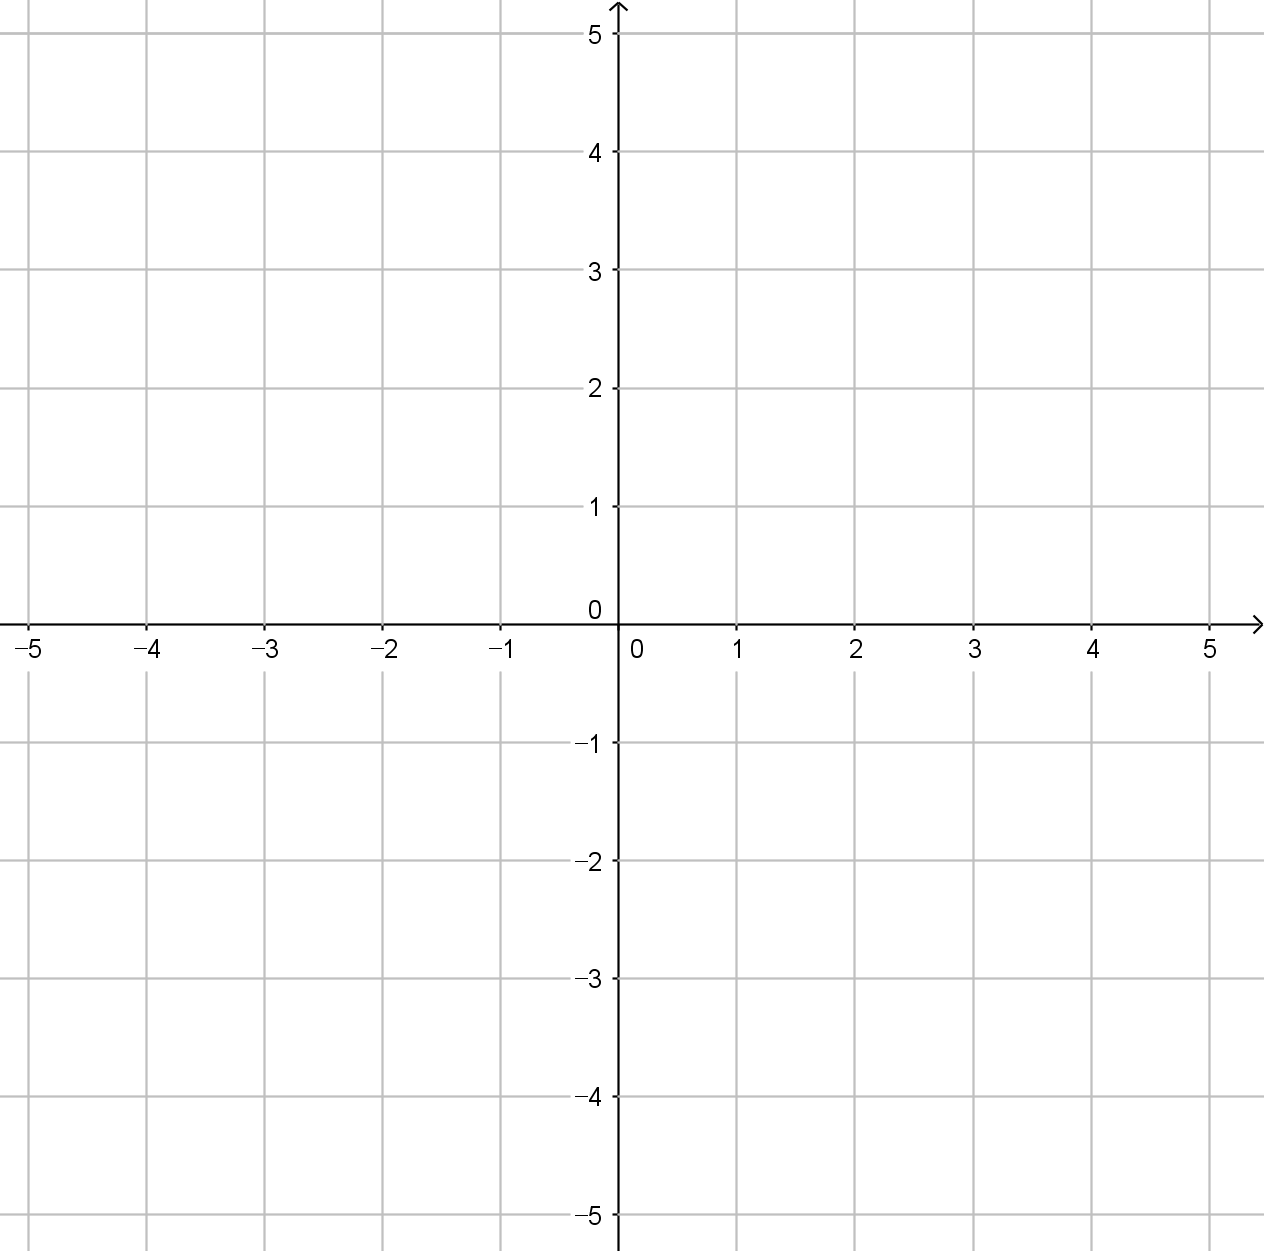
\includegraphics[width=\imagewidth]{55}
\end{minipage}\bigskip\bigskip\par

\newpage
\par\bigskip
j.두 점 $(2,1)$, $(4,5)$을 지나는 직선의 방정식을 구하여라.\par
\begin{minipage}{0.45\textwidth}\centering
\par\bigskip\begin{mdframed}
\vspace{\frameheight}
\end{mdframed}
\end{minipage}
\begin{minipage}{0.45\textwidth}\centering
\par\bigskip\par\bigskip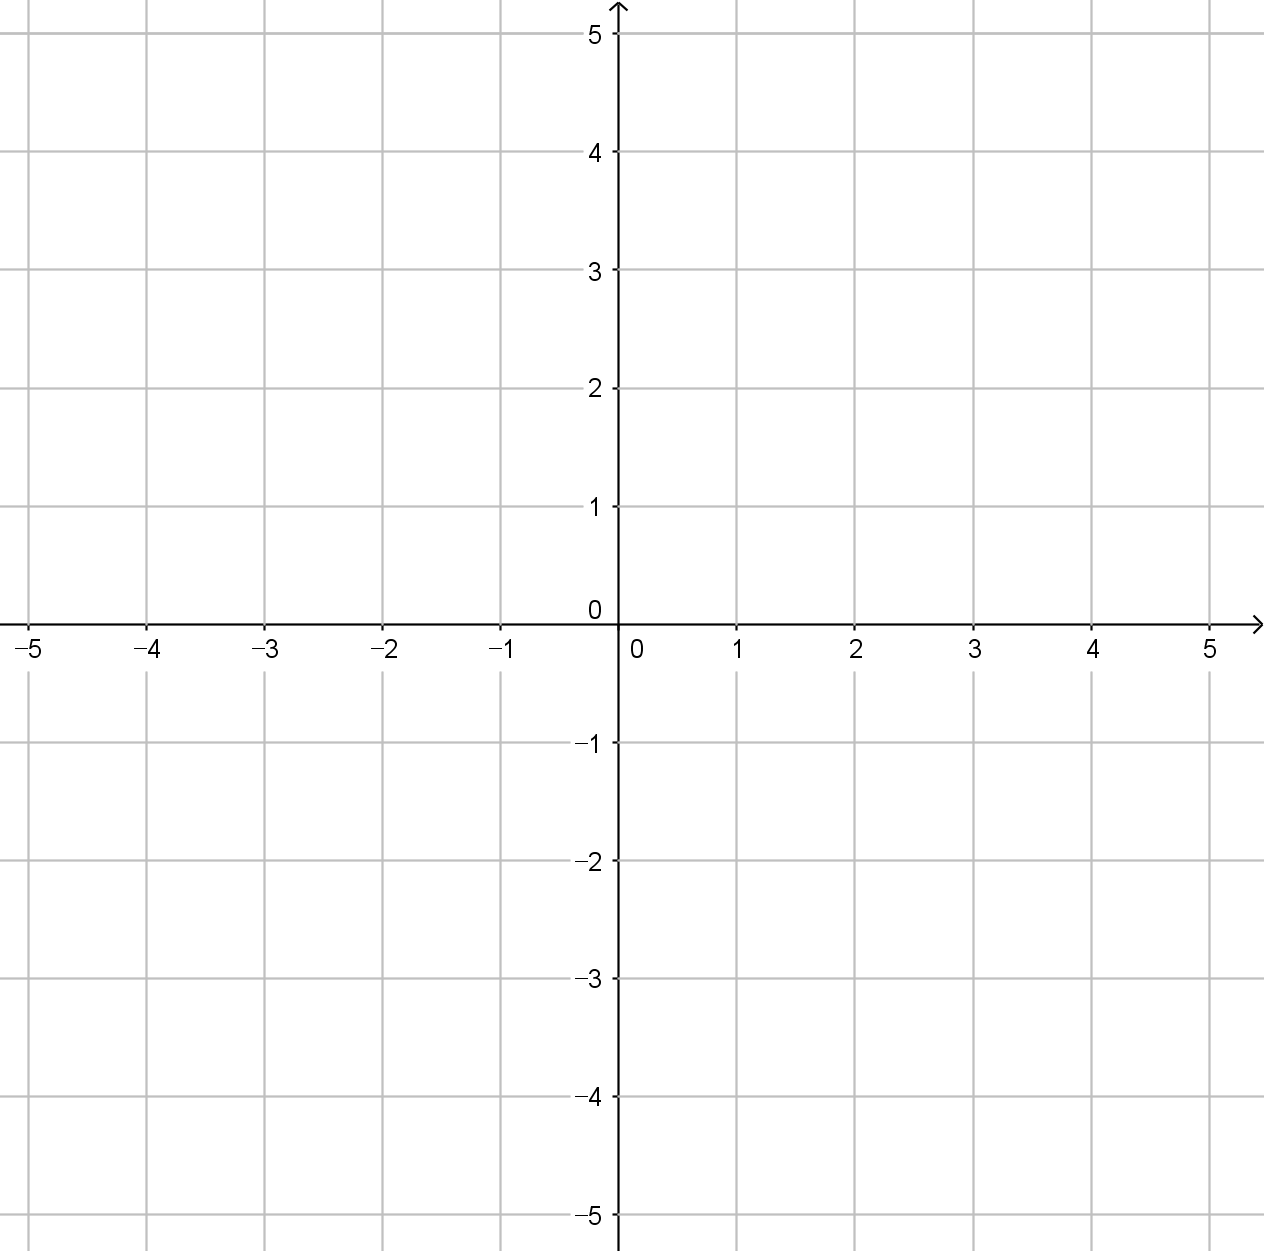
\includegraphics[width=\imagewidth]{55}
\end{minipage}\bigskip\bigskip\par
\par\bigskip
k,두 점 $(-2,-4)$, $(1,2)$을 지나는 직선의 방정식을 구하여라.\par
\begin{minipage}{0.45\textwidth}\centering
\par\bigskip\begin{mdframed}
\vspace{\frameheight}
\end{mdframed}
\end{minipage}
\begin{minipage}{0.45\textwidth}\centering
\par\bigskip\par\bigskip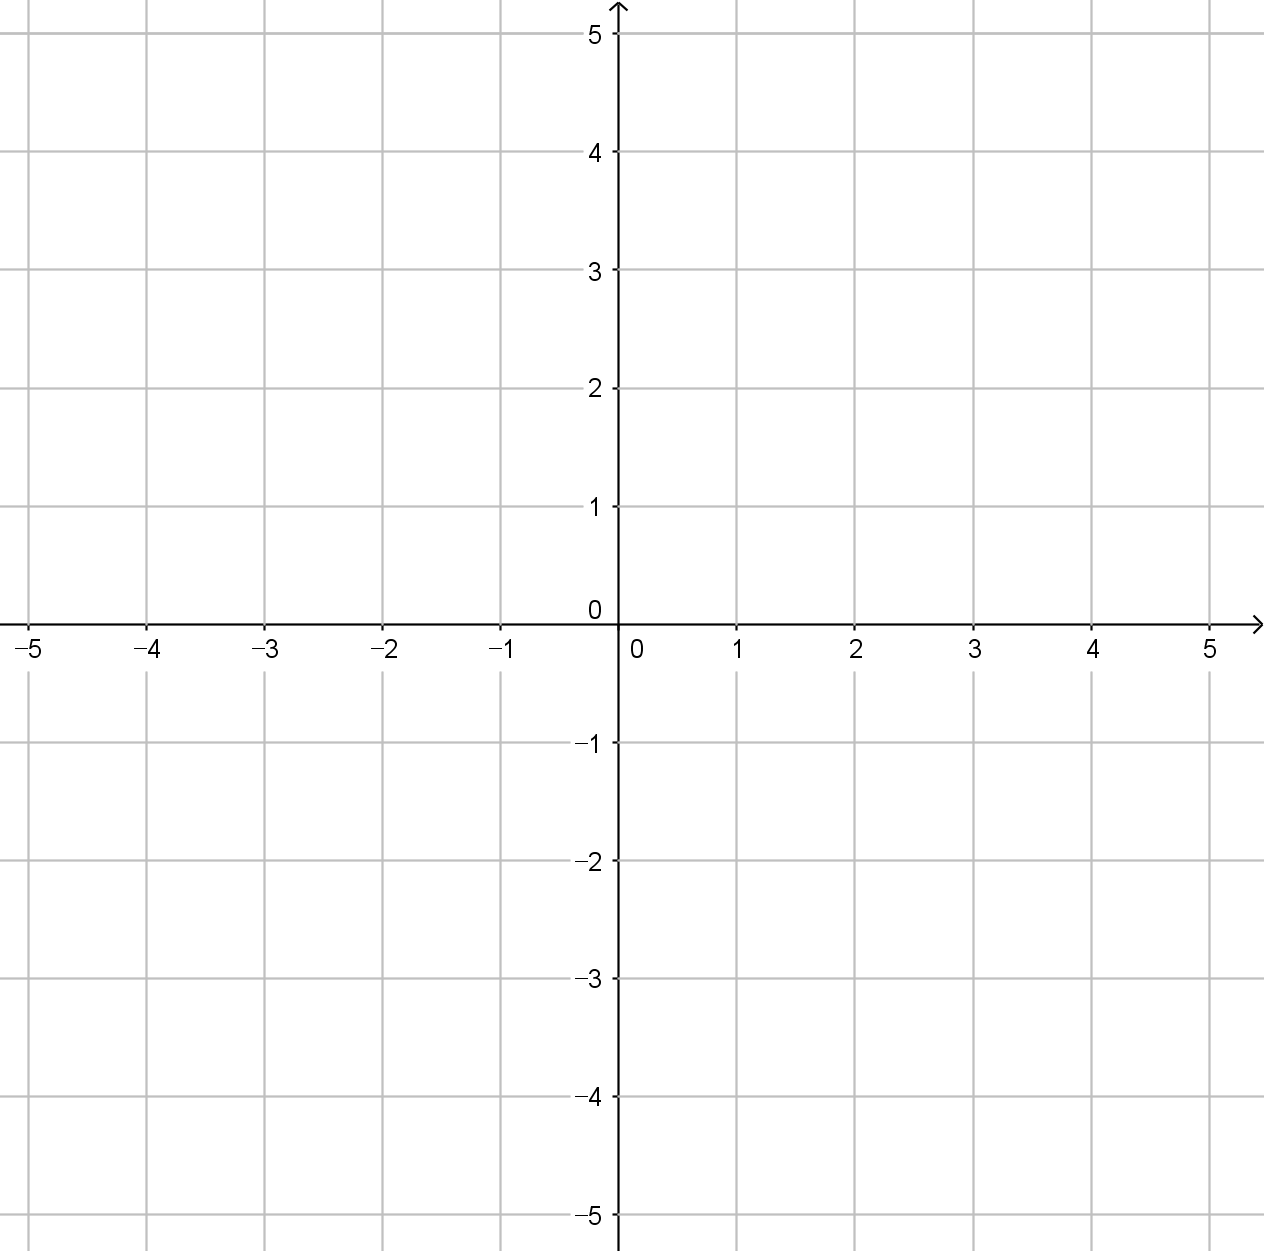
\includegraphics[width=\imagewidth]{55}
\end{minipage}\bigskip\bigskip\par
\par\bigskip
l.두 점 $(4,5)$, $(-2,2)$을 지나는 직선의 방정식을 구하여라.\par
\begin{minipage}{0.45\textwidth}\centering
\par\bigskip\begin{mdframed}
\vspace{\frameheight}
\end{mdframed}
\end{minipage}
\begin{minipage}{0.45\textwidth}\centering
\par\bigskip\par\bigskip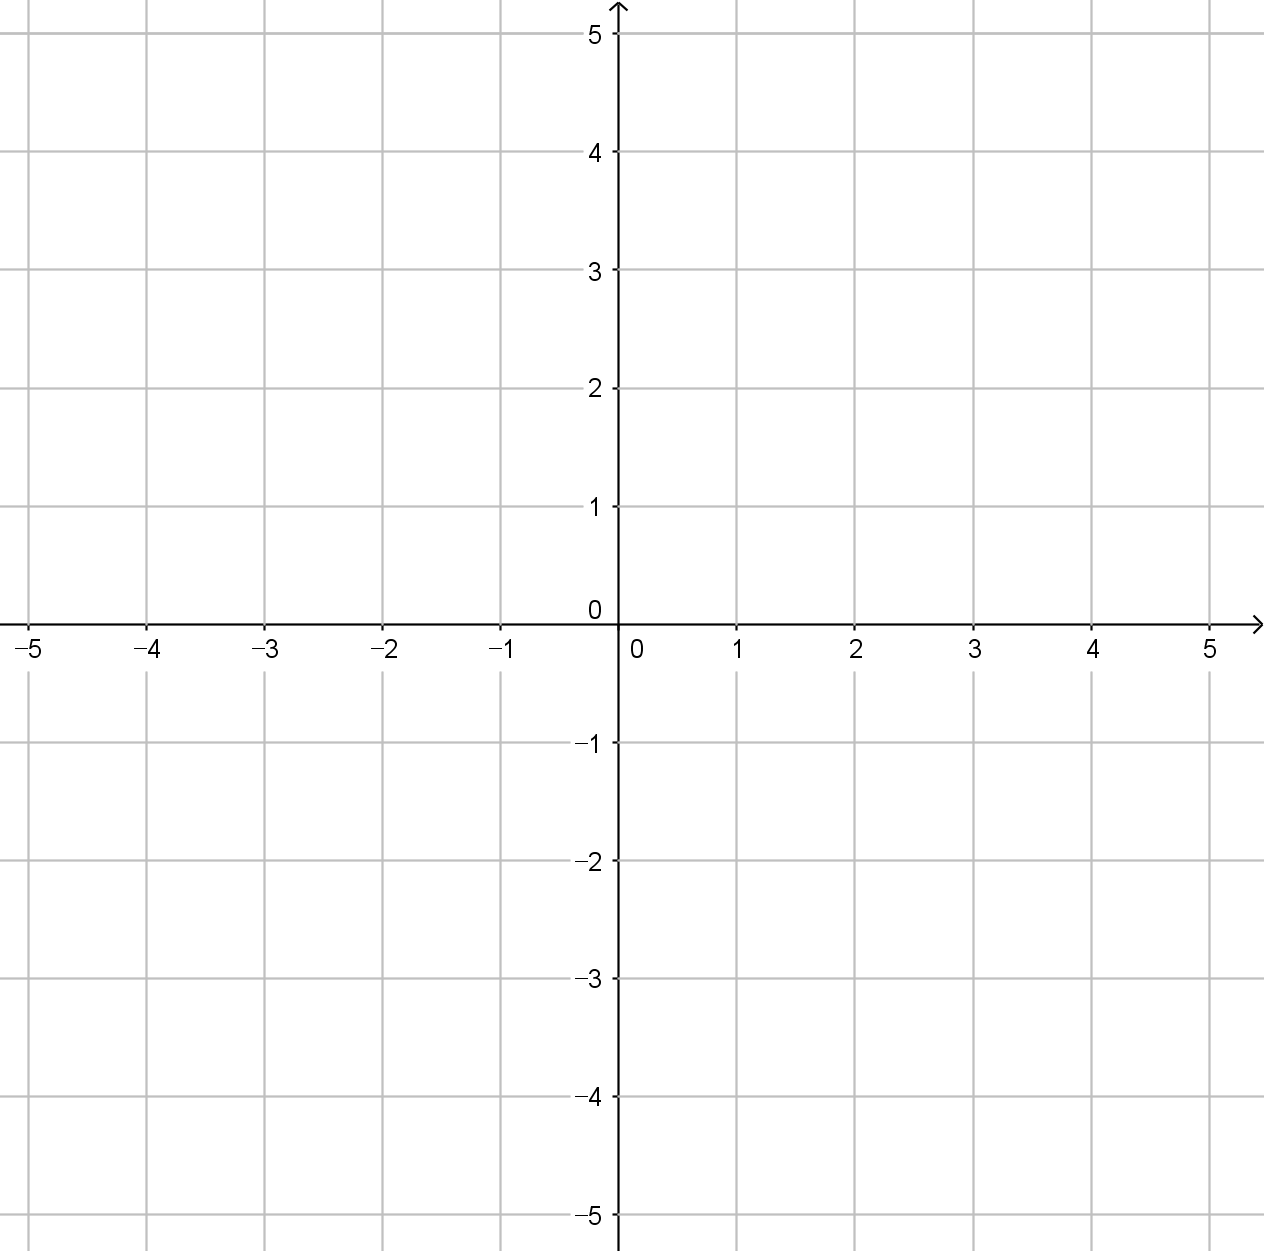
\includegraphics[width=\imagewidth]{55}
\end{minipage}\bigskip\bigskip\par
\end{document}